\chapter{Machine learning}\label{machineLearning}

Il capitolo spiega in breve la teoria dell'\textbf{apprendimento supervisionato} focalizzandosi nel contesto di regressione con processi gaussiani. Viene introdotto teoricamente il modello statistico che verrà usato, nel capitolo \ref{Capitolo: risultati training}, per produrre risultati legati al modello Windkessel visto nel capitolo \ref{windkessel}.\\
Le fonti usate per la stesura del capitolo sono: \cite{murphy_probabilistic_2022}, \cite{wiki:datasets}, \cite{wiki:overfitting}, \cite{pytorch:R2score}, \cite{wang_intuitive_2022}, \cite{noauthor_tutorial_nodate}, \cite{murphy_machine_2012}, \cite{gelman_bayesian_1995}, \cite{wiki:gradientDescend}, \cite{ruder_2022}, \cite{kingma_adam_2017}, \cite{JMLR:v12:duchi11a}, \cite{bottou2012stochastic}.


\begin{textblock*}{0.64\textwidth}(3.5cm+0.36\textwidth,18.5cm)
\epigraph{Il sole è sorto e tramontato per miliardi di anni. Il sole è tramontato anche stanotte. Con un'elevata probabilità, il sole domani sorgerà. Ma questo numero è molto più grande per colui che, vedendo nella totalità dei fenomeni il principio che regola i giorni e le stagioni, si rende conto che nulla al momento attuale può arrestarne il corso.}{Pierre Simon Laplace}
\end{textblock*}

\newpage

\section{Introduzione al machine learning}
Il \textbf{machine learning} (in italiano \textit{apprendimento automatico}) è una branca dell'\textbf{intelligenza artificiale}, la quale è una disciplina che studia i fondamenti teorici e le tecniche che consentono la progettazione di sistemi capaci di fornire all'elaboratore prestazioni che sembrerebbero essere di pertinenza esclusiva dell’intelligenza umana.\\
Di questa vasta branca, l'elaborato si interessa ai soli problemi di regressione, contrapposti ai problemi di classificazione.

In termini più pratici, il principale scopo del machine learning è lo studio e la costruzione di algoritmi che possano imparare a fare previsioni su dei dati. Tali algoritmi funzionano basandosi su decisioni guidate dal dataset  attraverso la costruzione di un modello matematico.\\
Nell'elaborato viene usato uno specifico tipo di apprendimento che è quello \textit{supervisionato}.

\begin{defi}[Apprendimento supervisionato]
L'\textbf{apprendimento supervisionato} è una tecnica di apprendimento automatico che mira a istruire un sistema informatico in modo da consentirgli di elaborare previsioni sulla base di una serie di esempi costituiti da coppie di input e output.
\end{defi}

\section{Dataset}\label{dataset}

Per ottimizzare la costruzione di algoritmi predittivi, i dati di input vengono divisi in più set di dati con ruoli diversi. Tipicamente viene usata una specifica partizione dei dati in tre dataset: \textbf{training}, \textbf{validation} e \textbf{test set}.


\begin{defi}[Training set]
Il \textbf{training set} è un insieme di esempi utilizzati durante il processo di apprendimento per determinare (o imparare) le combinazioni ottimali di parametri.
\end{defi}

In pratica, è sui dati del training set che viene eseguito il metodo di ottimizzazione scelto, aggiornando quindi i valori dei parametri o degli iperparametri.

\begin{defi}[Validation set]
Il \textbf{validation set} è un set indipendente di dati usato per valutare il modello addestrato sul training set.
\end{defi}
La valutazione (o \textit{validazione}) del modello sul validation set porta a decidere quali siano i migliori valori per i parametri (o iperparametri) in base alla performance sul validation set, appunto. Nel caso dell'elaborato viene usato un early-stopper, che sceglie come miglior modello quello con minore errore subito prima che si verifichi overfitting.

\begin{defi}[Test set]
Un \textbf{test set} è un set indipendente di dati dal training set  usato solo per valutare le prestazioni del modello.
\end{defi}

\newpage

Cioè il test set viene usato per valutare su un terzo set di dati indipendente il modello scelto in base alla performance sul validation set. Si ottengono così caratteristiche di prestazione come la precisione, la sensibilità, la specificità... Questo dataset è importante perché permette di valutare la performance del modello su un terzo insieme di dati indipendente dai precedenti evitando il rischio di overfitting: se un modello addestrato sul training test si adatta anche al test set, si è verificato un overfitting minimo.

È stato più volte citato il problema dell'\textbf{overfitting}, viene quindi riportata la definizione.

\begin{defi}[Overfitting]
L'\textbf{overfitting} è la generazione di un modello (o un'analisi) che corrisponde troppo strettamente a un particolare insieme di dati e può quindi non riuscire a prevedere osservazioni future in modo affidabile.
\end{defi}

L'overfitting può verificarsi per esempio includendo troppi parametri regolabili o usando un approccio troppo complicato, come mostrato in figura \ref{overfittigComplex}. Chiaramente, quando si confrontano diversi tipi di modelli la complessità deve tenere conto dell'influenza di ogni parametro sull'output\footnote{Si noti che si può incorrere nel problema opposto usando un approccio troppo semplice: l'underfitting. Ad esempio cercando di approssimare con una regressione lineare un campione con un andamento parabolico.}.

\begin{figure}[htbp]
    \centering
    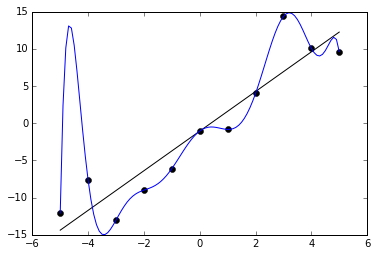
\includegraphics[width=0.6\textwidth]{images/Machine learning/Overfitted_Data.png}
    \caption{Esempio di overfitting. I dati (approssimativamente lineari) sono approssimati da una funzione lineare e da una polinomiale. Anche se la funzione polinomiale fornisce un adattamento quasi perfetto, ci si può aspettare che la funzione lineare generalizzi meglio i dati. \cite{wiki:overfitting}}
    \label{overfittigComplex}
\end{figure}

\newpage

L'overfitting è particolarmente probabile nei casi in cui l'apprendimento è stato eseguito troppo a lungo o in cui ci sono pochi dati per l'apprendimento, facendo sì che il modello si adatti a caratteristiche casuali molto specifiche dei dati di formazione che non hanno alcuna relazione causale con l'output. In questo caso di overfitting, la performance sul training set continua ad aumentare mentre la performance sul validation set peggiora, come mostrato in figura \ref{overfittingError}.



\begin{figure}[htbp]
    \centering
    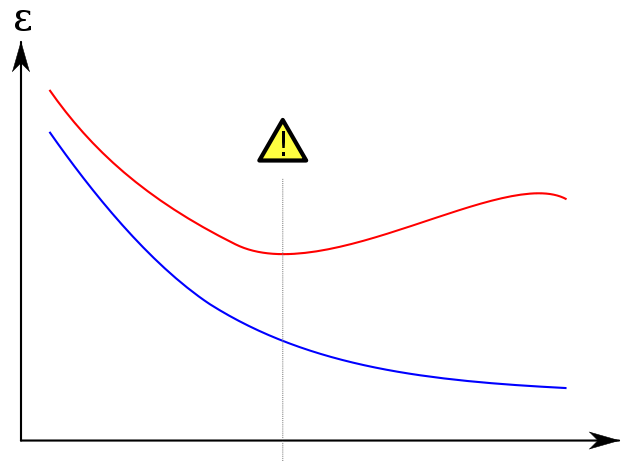
\includegraphics[width=0.6\textwidth]{images/Machine learning/Overfitting error.png}
    \caption{Overfitting nell'apprendimento supervisionato. Il training error (errore sul training set) è mostrato in blu, il validation error (errore su validation set) in rosso, entrambi in funzione del numero di cicli di training. \cite{wiki:overfitting}}
    \label{overfittingError}
\end{figure}


\subsection{Loss function}
Finora è stato delineato il problema che interessa l'elaborato: cercare una funzione $f$ per predire l'output $Y$ a partire dai valori dell'input $X$. Per farlo è necessaria una funzione di perdita, in inglese \textit{loss function}, $L(Y, f (X))$ per penalizzare gli errori di previsione.

\begin{defi}[Loss function]
Una \textbf{loss function} è una funzione in forma $\mathcal{L}(y_{\text{true}},y_{ \text{guess}})$ che definisce la perdita subita (o l'errore commesso) predicendo il valore $y_\text{guess}$ quando il valore vero è $y_{\text{true}}$,  fornendo quindi una valutazione delle capacità predittive del modello.
\end{defi}

Sarà questa la funzione da minimizzare con un algoritmo di ottimizzazione per l'adattamento degli iperparametri del processo gaussiano. Evidentemente la scelta della loss function dipende dal contesto.

%\section{Mean squared error}
%Per gli scopi dell'elaborato, si farà uso del \textit{mean squared error}.

%\begin{defi}[Mean squared error]
%Il \textbf{mean squared error} (o \textit{MSE}) è una \textit{loss function} definita come:
%\[
%\frac{1}{n}\sum^{n}_{i=1}(Y_i-f(X_i))^2,
%\]
%dove su $n$ dati raccolti, $Y_i$ sono gli output reali, $f(X_i)$ sono gli output predetti a partire da $X_i$.
%Poiché deriva dal quadrato della distanza euclidea, è sempre un valore positivo che diminuisce man mano che l'errore si avvicina a zero.
%\end{defi}
%Verrà usato non come loss function, ma per monitorare l'andamento del training.


%\section{Coefficiente di determinazione}
%Il coefficiente di determinazione fornisce una misura della bontà di adattamento di un modello, cioè quanto le previsioni di regressione approssimano i punti dei dati reali. Varia tra 0 e 1\footnote{Si possono apportare modifiche al coefficiente per fargli assumere anche altri valori, ma non vengono applicate nell'elaborato}, un $R^2$ di 1 indica che le previsioni di regressione si adattano perfettamente ai dati.

%Poichè il coefficiente di determinazione varia in un intervallo unitario, può essere più (intuitivamente) informativo di altre misure di errore (come il mean absolute error o il mean squared error) poiché tendono ad assumere valori su intervalli arbitrari oppure ad esprimere una percentuale.

%\begin{defi}[Coefficiente di determinazione]
%Date $y_i$ le osservazioni, $\overline{y}$ la media delle osservazioni, $\hat{y}_i$ i dati predetti dal modello:
%\[
%R^2 = 1-\frac{\sum_{i=1}^{n}(y_i-\hat{y}_i)}{\sum_{%i=1}^{n}(y_i-\overline{y})}
%\]
%\end{defi}
%Si noti che questo coefficiente non indica se:
%\begin{itemize}
%    \item una variabile sia statisticamente %significativa;
%    \item è stata usata la regressione corretta;
%    \item è stato scelto l'insieme più appropriato %di variabili indipendenti;
%    \item ci sono abbastanza dati per trarre una %conclusione solida.
%\end{itemize}

%Si noti inoltre che $R^2$ è una versione riscalata del mean squared error più facile da interpretare in quanto non dipende dalla scala dei dati.

\newpage
\section{Modelli parametrici e non parametrici}
Vi è una importante distinzione da fare sui modelli statistici: modelli parametrici e modelli non parametrici. Il tipo di modello, infatti, modifica notevolmente l'approccio teorico da usare e quindi i risultati applicativi. 


\subsection{Modelli parametrici}
I \textbf{modelli parametrici} presuppongono che la distribuzione dei dati possa essere modellata in termini di un insieme finito di parametri.\\
Un classico esempio è quello della regressione in cui, date delle osservazioni, si cerca di stimare un'eventuale relazione funzionale esistente tra la variabile dipendente e le variabili indipendenti. Se si assume un modello di regressione lineare, in cui la relazione è espressa dalla funzione $f(x) = \theta_1 + \theta_2x$ dove $x$ sono i dati di input, è necessario trovare i valori dei parametri $\theta_1$ e $\theta_2$ per definire $f$. In molti casi, l'assunzione del modello lineare non è sufficiente, ed è necessario un modello polinomiale (con più parametri): $f(x) = \theta_1+\theta_2x+\theta_3x^2$.\\
Quindi dato un dataset $D$ con $n$ punti osservati, dopo il processo di \textit{training} si assume che tutte le informazioni sulla relazione funzionale siano state catturate dai parametri $\theta_i$.  Quando si effettuano regressioni utilizzando modelli parametrici, la complessità e la flessibilità dei modelli è limitata dal numero di parametri. 

\subsection{Modelli non parametrici}
Contrariamente a quanto si possa pensare, un \textbf{modello non parametrico} non è un modello privo di parametri. \\
Intuitivamente, se il numero di parametri di un modello cresce con la dimensione del dataset di dati osservati, si tratta di un modello non parametrico. In via teorica, questo permette al modello di avere infiniti parametri e quindi di non dipendere da una struttura della funzione $f$ rigida, aumentandone la flessibilità.\\
Di interesse per l'elaborato è la regressione tramite processi gaussiani, che segue un approccio bayesiano non parametrico (visto nella sezione \ref{regressioneGP}). È in grado di \textit{apprendere} un'ampia varietà di  relazioni tra input e output utilizzando un numero teoricamente infinito di parametri e lasciando che i dati determinino il livello di complessità attraverso i mezzi di inferenza bayesiana.

Si veda \ref{gerarchica} per un chiarimento sulla differenza tra parametri e iperparametri nella regressione tramite processi gaussiani.

\newpage

\subsection{Struttura gerarchica}\label{gerarchica}
È comune usare una struttura gerarchica dei parametri e degli iperparametri nei modelli di regressione.

I parametri risiedono al livello più basso. Per esempio, nel caso della regressione lineare, i parametri sono i $\theta_i$, o nel caso di un modello di rete neurale i pesi associati ai neuroni.\\
Al secondo livello ci sono gli \textit{iperparametri} che controllano la distribuzione dei parametri al livello inferiore e dunque il cui valore è usato per controllare il processo di apprendimento.\\

Nel caso dei processi gaussiani, poiché sono un modello non parametrico, non è ovvio quali siano i parametri del modello. Si possono considerare come parametri i valori della funzione (priva di rumore) valutata sui dati osservati. Quindi sia $X=\{(x_i,y_i): i\in I\}$ l'insieme dei dati osservati, gli elementi $y_i$ possono essere considerati i parametri del modello. Evidentemente, più è grande $X$, più parametri ci sono. In termini pratici, si è visto in \ref{regressioneGP} come i dati osservati corrispondano alle informazioni sulla forma della funzione, quindi come la precisione dipenda dal numero di dati osservati.

È anche possibile dare una diversa lettura dei parametri del modello usando un'interpretazione teorica diversa (\textit{weight-space view}), che non è stata introdotta nell'elaborato.\footnote{Per approfondire: \cite{rasmussen_gaussian_2006}}\\

Gli iperparametri, invece, sono i parametri della mean function e della kernel function. Pragmaticamente, per fare regressione è necessario lavorare sulla stima degli iperparametri.


\newpage


\section{Ottimizzazione degli iperparametri}

\subsection{Inferenza bayesiana}
L'\textbf{inferenza bayesiana} è un metodo di inferenza statistica in cui il teorema di Bayes viene utilizzato per aggiornare la probabilità di un'ipotesi man mano che si rendono disponibili ulteriori  informazioni. 

Il processo bayesiano di analisi dei dati può essere idealizzato suddividendolo nelle seguenti tre fasi:
\begin{enumerate}
    \item Creazione di un modello di probabilità completo\\
    Il modello consiste in una distribuzione di probabilità congiunta per tutte le quantità relative al problema e deve essere coerente con le conoscenze del problema scientifico di base.
    \item Condizionamento dei dati osservati\\ Viene calcolata e interpretata l'appropriata distribuzione a posteriori, ovvero la distribuzione di probabilità delle quantità non osservate condizionata rispetto i dati osservati.
    \item Valutazione dell'adattamento del modello\\
    Viene valutato quanto il modello si adatta ai dati e se le conclusioni sostanziali sono ragionevoli. In questa fase è possibile modificare o espandere il modello e ripetere le tre fasi.
\end{enumerate}
L'approccio bayesiano può essere interpretato come una formalizzazione del metodo scientifico, in cui si cerca di aggiornare la conoscenza scientifica attraverso esperimenti e osservazioni.\\
Inoltre, questo approccio statistico gode di una flessibilità tale da essere utilizzabile in problemi complessi, anche con molti parametri.\\

Nell'ambito dei processi gaussiani viene studiato l'uso dell'inferenza bayesiana nell'ottimizzazione degli iperparametri.

\newpage

\subsection{Teorema di Bayes}
\begin{teo}[Teorema di Bayes]
Siano $A, B$ eventi, sia $\probP(B)\neq 0$, allora:
\[
\probP(A|B) = \frac{\probP(B|A)\probP(A)}{\probP(B)}.
\]
\end{teo}
\begin{proof}
Dalla definizione di probabilità condizionata si ha: $\probP(A\cap B) = \probP(A|B)\probP(B)$, da cui segue $\probP(A|B)=\frac{\probP(A\cap B)}{\probP(B)}$ se $\probP(B)\neq 0$; analogamente: $\probP(B|A)=\frac{\probP(A\cap B)}{\probP(A)}$ se $\probP(A)\neq 0$. Sostituendo $\probP(A\cap B)$ nell'espressione di $\probP(A|B)$ si conclude.
\end{proof}

\vspace{0.5cm}

Nel contesto bayesiano lo scopo dell'analisi di un modello è quello di trarre conclusioni statistiche su un parametro $\theta$ (o analogamente su un vettore di parametri\footnote{Per il momento viene preso in considerazione il caso dei parametri, ma quanto detto si estende immediatamente al caso degli iperparametri, come visto in \ref{evidenzaBayesiana}}) o su dati non osservati; le suddette conclusioni vengono formulate in termini di probabilità condizionate al valore osservato di $y$. 
Per poter fare affermazioni di probabilità su $\theta$ osservati i dati $y$ è necessario iniziare con un modello che fornisca una distribuzione di probabilità congiunta per $\theta$ e $y$, fattorizzabile in due componenti: $\probP(\theta)$, cioè la distribuzione a priori che descrive la conoscenza sulla distribuzione di $\theta$ prima di osservare i dati, e $\probP(y|\theta)$, cioè la distribuzione dei dati (o campionaria):
\[
\probP(\theta, y)=\probP(\theta)\probP(y|\theta).
\]

Applicando il teorema di Bayes si ottiene la \textit{distribuzione a posteriori}:
\[
\probP(\theta | y)=\frac{\probP(\theta)\probP(y|\theta)}{\probP(y)},
\]
nella quale il denominatore può essere riscritto, per il teorema della probabilità assoluta (in inglese \textit{law of total probability}), come:
\[
\probP(y)=\begin{cases}\sum_\theta \probP(\theta)\probP(y| \theta)\\\int\probP(\theta)\probP(y| \theta)d\theta \end{cases} \text{ in base a }\theta.
\]
Poiché $\probP(y)$ non dipende da $\theta$ e fissando $y$ è possibile riscrivere la distribuzione a posteriori come:

\[
\probP(\theta | y)\propto \probP(\theta)\probP(y|\theta),
\]
dove, avendo fissato $y$, $\probP(y|\theta)$ è funzione di $\theta$.

\newpage

\subsection{Evidenza bayesiana}\label{evidenzaBayesiana}
Nel contesto dei modelli statistici, la reinterpretazione del teorema di Bayes (e di quanto detto nella sezione precedente) è:
\[
\probP(\theta | X, \alpha) = \frac{\probP(X|\theta, \alpha)\probP(\theta | \alpha)}{\probP(X|\alpha)}\propto \probP(\theta | \alpha) \probP(X|\theta, \alpha),
\]
dove: $\theta$ è il vettore di parametri, $\alpha$ il vettore degli iperparametri, $X$ il campione di dati osservati. In questo caso la distribuzione a priori è composta da $\probP(\theta|\alpha)$\footnote{Si noti che è condizionata rispetto al valore degli iperparametri. Questo è dovuto alla definizione degli iperparametri, che controllano la distribuzione dei parametri, come detto nella sezione \ref{gerarchica}.}, la distribuzione dei parametri prima di osservare i dati $X$; $\probP(X|\theta)$, la distribuzione campionaria che è la distribuzione dei dati osservati condizionata al valore dei parametri; e $\probP(X|\alpha)$, l'\textbf{evidenza} (anche chiamata \textit{verosimiglianza marginale}, in inglese \textit{marginal likelihood}) che è la distribuzione dei dati condizionata rispetto gli iperparametri. Quest'ultima è possibile riscriverla come
\[
\probP(X|\alpha) = \int \probP(X|\theta)\probP(\theta | \alpha)d\theta,
\]
cioè come la distribuzione dei dati marginalizzata sui parametri.

Oltre ad essere il termine di normalizzazione nel teorema di Bayes, un possibile altro modo di interpretare la marginal likelihood è quello di considerarla la probabilità di aver generato il dataset (osservato) $X$ dati gli iperparametri $\alpha$.

Utilizzando ancora il teorema di Bayes si ottiene:
\[
\probP(\alpha |X) = \frac{\probP(X|\alpha)\probP(\alpha)}{\probP(X)}\propto \probP(X|\alpha) \probP(\alpha),
\]
cioè la distribuzione a posteriori (che rappresenta la distribuzione degli iperparametri osservati i dati $X$) è proporzionale alla marginal likelihood. Poiché nel caso preso in considerazione dall'elaborato, cioè i processi gaussiani, uno degli obiettivi è trovare la distribuzione degli iperparametri (cioè la forma della covariance function, in altri termini $\probP(\alpha|X)$), l'approccio adottato è quello di massimizzare la marginal likelihood, sfruttando la dipendenza evidenziata nella formula precedente. Questo approccio è chiamato \textbf{evidence approach}.

\newpage

\subsection{Alternative all'evidenza bayesiana}
La scelta dell'approccio per stimare il valore di parametri o iperparametri dipende molto dalla situazione. Ad esempio:
\begin{itemize}
    \item Massimizzazione della \textit{likelihood}:
    si massimizza $L(\alpha, \theta | X)$ (la funzione di verosimiglianza), dunque si trovano valori di $\alpha$ e  $\theta$ che la massimizzano;
    \item Massimizzazione parziale della \textit{likelihood}:
    dato il caso in cui $L(\alpha, \theta |X)=L_1(\alpha | X)L_2(\theta|X)$, si massimizza solo il fattore di interesse, nel caso in esame si massimizza $L_1(\alpha | X)$;
    \item Massimizzazione della \textit{marginal likelihood}:
    si marginalizza su $\theta$, quindi si massimizza $\probP(X|\alpha)$ che dipende solo da $\alpha$.
\end{itemize}
L'elaborato applica l'ultimo caso poiché i calcoli necessari sono tutti analiticamente risolubili. In altre situazioni questo approccio richiede un'approssimazione numerica che può portare a problemi di stabilità, motivo per cui non è sempre un approccio usato.




\subsection{Nei processi gaussiani}\label{neiProcessiGaussiani}
L'approccio che i processi gaussiani seguono è quello di definire una \textit{distribuzione sulle funzioni} (in inglese \textit{distribution over functions}), aggiornarla a partire dai dati osservati e usarla per fare previsioni su nuovi input. \\
Si consideri quanto fatto nella sezione \ref{noisyPrediction}: si è definita una distribuzione a priori sulle funzioni che poi è stata convertita in una distribuzione a posteriori aggiornando le informazioni grazie ai dati osservati. A differenza del caso \textit{noise-free}, però, non si ottiene una funzione che interpoli perfettamente i dati. In questo caso è dunque necessario scegliere opportuni iperparametri, in modo da ottimizzare la forma della funzione: questa stima viene fatta tramite evidence approach sfruttando il fatto che le espressioni degli integrali sono tutte analiticamente risolubili.\\


In questo caso la marginal likelihood è:
\[
\probP(\bf{y}|\bf{\alpha}) = \int \probP(\bf{y}| \mathbf{f},\bf{\alpha})\probP(\mathbf{f}|\bf{\alpha}) d\mathbf{f},
\]

dove $\bf{\alpha}$ sono gli iperparametri, $\mathbf{f}$ sono dati osservati senza errore (sono i parametri), $\bf{y}$ sono i dati osservati.\\
Si noti che $\probP(\mathbf{f}|\bf{\alpha})$ è la distribuzione a priori della funzione priva di errori ed è una distribuzione gaussiana multivariata in quanto $\mathbf{f}|\alpha\sim \mathcal{N}(m, K)$ con $K$ la matrice di Gram della covariance function e $m$ la valutazione della mean function sul vettore di input. Inoltre, dalla definizione di $\mathbf{y}$ si ha $\mathbf{y}|\mathbf{f}\sim \mathcal{N}(\mathbf{f}, \sigma_n^2I)$, dove $\epsilon\sim \mathcal{N}(0,\sigma_n^2)$.

\newpage

Con i calcoli riportati su \cite{rasmussen_gaussian_2006} si conclude:
\[
L=\text{log}(\probP(\mathbf{y}|\alpha))=-\frac{1}{2}\text{log}(|K+\sigma_n^2I|)-\frac{1}{2}(\mathbf{y}-m)^{\text{T}}(K+\sigma_n^2I)^{-1}(\mathbf{y}-m)-\frac{n}{2}\text{log}(2\pi)
\]

Lo stesso risultato si può ottenere evitando i conti analitici notando: $\mathbf{y}\sim \mathcal{N}(m, K+\sigma_n^2I)$. A questo punto è semplice calcolare le derivate parziali rispetto agli iperparametri della covariance function e della mean function. Questo è di fondamentale importanza per i metodi numerici di ottimizzazione.

Si noti che la massimizzazione della marginal likelihood è preferibile rispetto alla massimizzazione della likelihood (o altri metodi di likelihood) poiché con altre forme di likelihood è possibile ottenere un overfitting (si veda \ref{dataset} per la definizione di overfitting). Al contrario, la marginal likelihood non esegue un \textit{fitting} dei valori delle funzioni, ma li integra (li marginalizza), cioè tecnicamente non può fare overfitting perché non avviene alcun \textit{fit}. \\

Per ulteriori considerazioni, dettagli sui conti e approfondimenti su come ottimizzare i calcoli numerici si rimanda a \cite{rasmussen_gaussian_2006}.




\section{Metodo di ottimizzazione}
L'\textbf{ottimizzazione} è la branca della matematica che studia teoria e metodi per la ricerca dei punti di massimo e minimo di una funzione. Questa sezione si ripropone di ripercorrere i principali passi teorici che hanno portato alla costruzione del metodo di ottimizzazione usato successivamente nella massimizzazione della marginal likelihood: Adam.

\subsection{Forma della funzione da ottimizzare}\label{costfunction}
Per comprendere la differenza tra i metodi di ottimizzazione che vengono riportati è importante comprendere la forma della funzione da ottimizzare.
Nell'ambito dell'apprendimento supervisionato si ha un dataset di osservazioni da cui si vuole imparare. Per farlo, in breve, si definisce una funzione che rappresenta l'errore che il nostro modello compie sul dataset di valori osservati\footnote{Si veda la sezione \ref{dataset}, in cui viene spiegato come dividere un dataset in sottoinsiemi con diversi ruoli.}: l'obiettivo è minimizzare questa funzione e per farlo è necessario, usando un opportuno algoritmo, cambiare i valori dei parametri (nel caso in esame, un modello non parametrico, vengono modificati gli iperparametri).

\newpage

Siccome il dataset di dati osservati conterrà potenzialmente molti dati, è necessario tenere conto dell'errore commesso valutandolo in ogni dato osservato. Generalmente, infatti, la funzione di errore ha forma:
\[
Q(w)=\sum_{i=1}^{n}Q_i(w),
\]
dove tendenzialmente ogni addendo dipende da un singolo dato del dataset di input. Un esempio è:
\[
f(m,b)=\sum_{i=1}^{N}(y_i-(mx_i+b))^2,
\]
cioè il metodo dei minimi quadrati nella regressione lineare.\\
Si noti che nel caso in esame la funzione da ottimizzare, la marginal likelihood, è una somma in cui l'addendo $i$-esimo non dipende solo dall'$i$-esimo dato osservato.


\subsection{Learning rate}
I metodi iterativi di ottimizzazione hanno una forma simile tra loro: dato $\theta_0$ punto iniziale, ad ogni iterazione si aggiorna il punto come:
\[
\theta_{t+1}=\theta_t+\eta_td_t,
\]
dove $d_t$ rappresenta una direzione ed è definita in base al metodo, $\eta_t$ è la lunghezza del passo (in inglese \textit{step size}) o \textit{learning rate} e indica di quanto ci si sposta nella direzione $d_t$. Il learning rate può essere costante oppure può essere aggiornato ogni iterazione.


\newpage

\subsection{Metodo del gradiente \cite{ruder_2022}}
Il \textbf{metodo del gradiente} sfrutta il fatto che il gradiente è la direzione di massima crescita della funzione. Ha forma:
\begin{align*}
    &\text{Dato un valore iniziale }\omega_0, \eta_0\\
    &\text{Da ripetere fino a che si trova un'approssimazione del minimo:}\\
    &\quad \omega_{k+1}=\omega_k - \eta_k\cdot \nabla Q(\omega_k).
\end{align*}
Con "\textit{Da ripetere fino a che si trova un'approssimazione del minimo}" si intende che si ripete il metodo fino a che non viene soddisfatta una condizione di uscita che incorpora la precisione che si chiede all'approssimazione.\\
Poiché, come visto in \ref{costfunction}, è necessario valutare il gradiente su ogni elemento del dataset, può essere un metodo oneroso soprattutto in termini di memoria.\\
Il learning rate $\eta_k$ può essere costante per ogni $k$ oppure può essere modificato ad ogni iterazione. In entrambi i casi svolge un ruolo importante poiché può portare, se troppo piccolo, ad una convergenza troppo lenta oppure, se troppo grande, ad una divergenza. Nel caso di un learning rate aggiornato ad ogni iterazione, generalmente lo si diminuisce mano a mano che ci si avvicina al minimo; ad esempio si veda la figura \ref{gradientDescentImage}.

\begin{figure}[h]
    \centering
    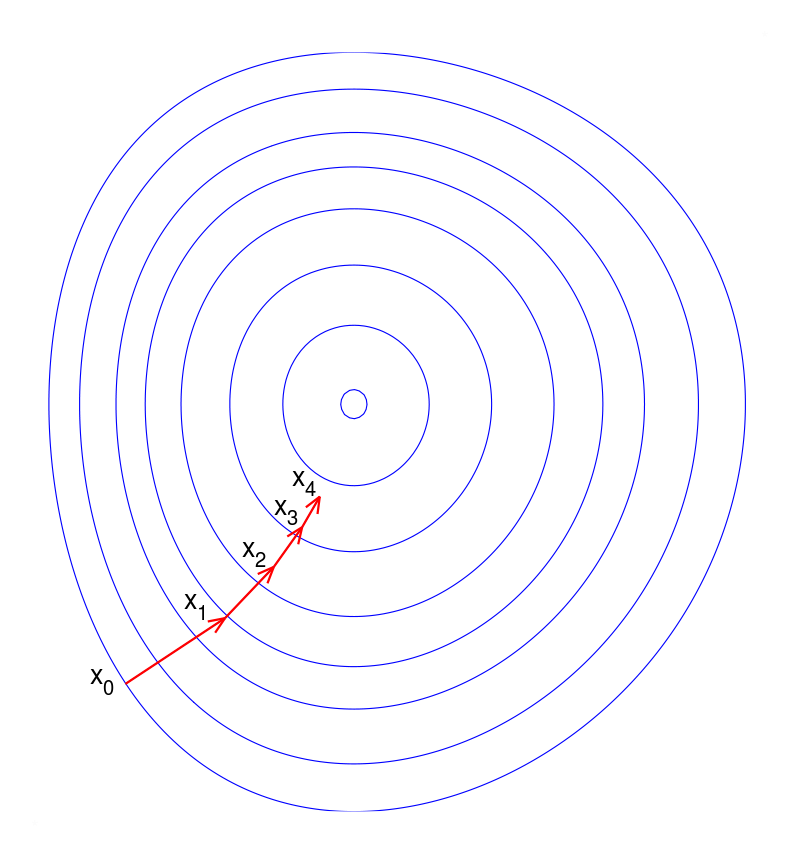
\includegraphics[width=0.6\textwidth]{images/Training (teoria)/Gradient descend.png}
    \caption{Illustrazione del metodo del gradiente su degli insiemi di livello, ad ogni iterazione viene aggiornato il learning rate.\cite{wiki:gradientDescend}}
    \label{gradientDescentImage}
\end{figure}



\subsection{Discesa stocastica del gradiente \cite{bottou2012stochastic}}
Il metodo di \textbf{discesa stocastica del gradiente}, diversamente dal metodo del gradiente, esegue un aggiornamento per ogni $Q_i$\footnote{Nel caso in cui la $Q$ si scriva come somma di termini che dipendono ognuno solo da un elemento del dataset, comporta che il metodo esegue un aggiornamento per ogni elemento del dataset.}. Ha forma:
\begin{align*}
    &\text{Dato un valore iniziale }\omega_0, \eta_0\\
    &\text{Da ripetere fino a che si trova un'approssimazione del minimo:}\\
    &\quad\text{Mescola il dataset}\\
    &\quad\text{Per }i=1,...,n:\\
    &\quad\quad\omega_{k+1}=\omega_k -\eta_k\cdot \nabla Q_i(\omega_k)
\end{align*}
Dovendo calcolare il gradiente per un solo addendo di $Q$ alla volta, è un metodo molto più veloce, seppur questi frequenti aggiornamenti causino un'alta fluttuazione della funzione obiettivo, come si può notare dalla figura \ref{MomentumMethod}.\\
Anche se la fluttuazione può sembrare uno svantaggio del metodo, è proprio questa che gli permette di evitare minimi locali e tendere a migliori approssimazioni. Il metodo del gradiente visto precedentemente invece converge al minimo del bacino in cui è stato scelto il dato iniziale.\\
D'altra parte, la fluttuazione complica la convergenza verso il minimo esatto a causa dei frequenti cambiamenti che la funzione subisce. Tuttavia è stato dimostrato che quando si diminuisce lentamente il learning rate il metodo mostra lo stesso comportamento di convergenza del metodo del gradiente. 


\newpage
\subsection{Metodo dei momenti \cite{ruder_2022}}
Il metodo stocastico del gradiente ha difficoltà a percorrere i \textit{burroni}, cioè le aree in cui la superficie curva più ripidamente in una dimensione rispetto a un'altra. In questi scenari, il metodo oscilla lungo le pendici del burrone, mentre progredisce con esitazione lungo il fondo verso il minimo, come mostrato nella figura \ref{MomentumMethod}.\\
Il \textbf{metodo dei momenti} è un metodo che aiuta ad accelerare il metodo stocastico del gradiente nella direzione desiderata e a smorzare le oscillazioni, come si vede nella figura \ref{MomentumMethod}. Ha forma:

\begin{align*}
    &\text{Dato un valore iniziale }\omega_0, \eta_0, v_0=0\\
    &\text{Da ripetere fino a che si trova un'approssimazione del minimo:}\\
    &\quad\text{Mescola il dataset}\\
    &\quad\text{Per }i=1,...,n:\\
    & \quad\quad v_t=\gamma v_{t-1}+\eta_k\cdot \nabla Q_i(\omega_k)\\
    &\quad\quad\omega_{k+1}=\omega_k - v_t
\end{align*}
Il termine di $\gamma$ è chiamato \textit{momento} (o \textit{quantità di moto}) ed è solitamente impostato a 0.9.\\
In sostanza quello che avviene è analogo a quando si spinge una palla giù per una collina: la palla accumula quantità di moto
mentre rotola in discesa  diventando sempre più veloce (finché non raggiunge la sua velocità terminale, se c'è
la resistenza dell'aria, cioè $\gamma<1$). La stessa cosa accade agli aggiornamenti dei parametri: nel vettore il termine di "quantità di moto" favorisce le dimensioni in cui il gradiente punta nella stessa direzione e sfavorisce le altre. Di conseguenza, si ottiene una convergenza più rapida e una riduzione dell'oscillazione, riducendo i problemi del metodo stocastico del gradiente, come si mostra in figura \ref{MomentumMethod}.

\begin{figure}[h]
\centering
\begin{subfigure}{.5\textwidth}
  \centering
  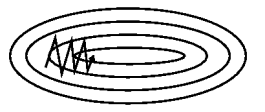
\includegraphics[width=\linewidth]{images/Training (teoria)/SGD Momentum a.PNG}
  \caption{Senza momento.}
\end{subfigure}%
\begin{subfigure}{.5\textwidth}
  \centering
  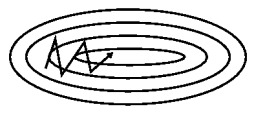
\includegraphics[width=\linewidth]{images/Training (teoria)/SGD Momentum b.PNG}
  \caption{Con momento.}
\end{subfigure}
\caption{Metodo dei momenti applicato al metodo stocastico del gradiente. \cite{ruder_2022}}
\label{MomentumMethod}
\end{figure}

\newpage
\subsection{AdaGrad \cite{JMLR:v12:duchi11a}}
Il metodo \textbf{AdaGrad} (abbreviazione di \textit{Adaptive Gradient algorithm})  è un algoritmo di ottimizzazione basato sul metodo stocastico del gradiente che usa un learning rate indipendente per ogni $\omega_i$. Per i termini $\omega_i$ che hanno gradiente più elevato o aggiornamenti frequenti, il metodo impone un learning rate più basso, in modo da non superare il minimo. Viceversa quelli con gradiente basso o aggiornamenti poco frequenti avranno un learning rate più alto, in modo da essere addestrati rapidamente.\\



Adagrad migliora la robustezza del metodo stocastico del gradiente e converge più rapidamente soprattutto quando la distribuzione dei dati è sparsa; ha dimostrato ottimi risultati nell'addestramento di reti neurali su larga scala (ad esempio in Google).

\begin{align*}
    &\text{Dato un valore iniziale }\omega_0, \eta\\
    &\text{Da ripetere fino a che si trova un'approssimazione del minimo:}\\
    &\quad\text{Mescola il dataset}\\
    &\quad\text{Per }i=1,...,n:\\
    &\quad\quad \text{Per ogni componente $j$ di $\omega$:}\\
    &\quad\quad\quad g_{k,j}=(\nabla Q_i(\omega_k))_j\\
    &\quad\quad\quad\omega_{k+1,j}=\omega_{k,j} - \frac{\eta}{\sqrt{G_{k,j}}+\epsilon}g_{k,j}
\end{align*}
Dove $G_{k,j}=\sum_{t=1}^{k}g_{t,j}^2$ e $\epsilon$ un termine piccolo per evitare divisioni per zero (generalmente $10^{-8}$).\\
Poiché adatta il learning rate, uno dei principali vantaggi del metodo è che elimina la necessità di regolare manualmente $\eta_k$: generalmente si imposta $\eta=0,01$.\\
Il punto debole di Adagrad è l'accumulo dei gradienti al quadrato nel denominatore: poiché ogni termine aggiunto è positivo, la somma accumulata continua a crescere durante l'addestramento. Questo fa sì che il learning rate si riduca e tenda a diventare infinitesimamente piccolo, a quel punto l'algoritmo non è più in grado di acquisire ulteriori conoscenze.


\newpage
\subsection{Adam \cite{kingma_adam_2017}}\label{adam}
Il metodo \textbf{Adam} (abbreviazione di \textit{Adaptive Moment Estimation}) è, come il precedente, un metodo a learning rate adattivi per ogni parametro. Deriva da altri metodi (AdaDelta, RMSprop) che cercano di ridurre il tasso di apprendimento monotonicamente decrescente del metodo AdaGrad. Infatti: invece di accumulare tutti i gradienti passati al quadrato, la somma dei gradienti è ricorsivamente definita come una media decrescente di tutti i gradienti quadratici passati, che dipende quindi dalla media precedente e dal gradiente corrente, ed è chiamata $v_k$. Inoltre, il metodo di Adam prevede la stessa media decrescente dei gradienti passati, chiamata $m_k$.


\begin{align*}
    &\text{Dato un valore iniziale }\omega_0, \eta, m_0=0, v_0=0\\
    &\text{Da ripetere fino a che si trova un'approssimazione del minimo:}\\
    &\quad\text{Mescola randomicamente il dataset}\\
    &\quad\text{Per }i=1,...,n:\\
    &\quad\quad \text{Per ogni componente $j$ di $\omega$:}\\
    &\quad\quad\quad g_{k,j}=(\nabla Q_i(\omega_k))_j\\
    &\quad\quad\quad m_k=\beta_1m_{k-1}+(1-\beta_1)g_{k,j}\\
    &\quad\quad\quad v_k=\beta_2v_{k-1}+(1-\beta_2)g^2_{k,j}\\
    &\quad\quad\quad \hat{m}_k = \frac{m_k}{1-\beta_1^k}\\
    &\quad\quad\quad \hat{v}_k = \frac{v_k}{1-\beta_2^k}\\
    &\quad\quad\quad\omega_{k+1,j}=\omega_{k,j} - \frac{\eta}{\sqrt{\hat{v_k}}+\epsilon}\hat{m_k}
\end{align*}
I termini $m_k$ e $v_k$, le medie decrescenti dei gradienti e dei gradienti quadrati, sono stime del primo momento e del secondo momento dei gradienti, come definito nel metodo dei momenti. Poiché  $m_k$ e $v_k$ sono distorti verso valori prossimi allo zero, si usano stimatori corretti $\hat{m}_k$ e $\hat{v}_k$. Generalmente si impongono valori $\beta_1=0.9$ e $\beta_2=0.999$.

\newpage
In figura \ref{comparison} vengono comparati alcuni metodi nella minimizzazione della cost function in una neural network. Si nota che il metodo di Adam è molto più efficiente degli altri metodi introdotti nell'elaborato.
\begin{figure}[h]
    \centering
    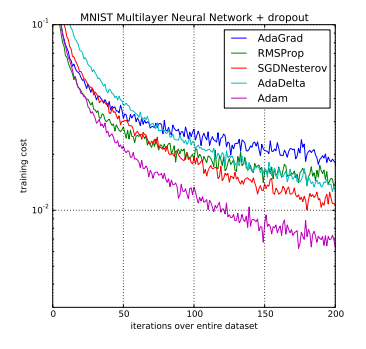
\includegraphics[width=0.75\textwidth]{images/Machine learning/Comparison.PNG}
    \caption{Comparazione di metodi di minimizzazione di una cost function in una rete neurale. \cite{kingma_adam_2017}}
    \label{comparison}
\end{figure}